\section{Исследование}

Исследование проводилось на основе таблиц, содержащих от 1000 до 11 000 записей с шагом 1000. Количество итераций сортировок: 10. Все данные были сгенерированы случайным образом. В ходе эксперимента применялись два алгоритма сортировки: классическая сортировка пузырьком и её улучшенная версия — сортировка пузырьком с флагом. Замеры производительности выполнялись как для сортировки всей таблицы целиком, так и для сортировки ключей.

\begin{figure}[H]
	\centering
	\includegraphics[width=0.94\textwidth]{img/linear_time_buble.jpg}
	\captionsetup{font=footnotesize}
	\caption{Зависимость времени между сортировкой стран и ключей при сортировке пузырьком}
	\label{fig:01}
\end{figure}

\begin{table}[H]
	\begin{longtable}{|c|c|c|}
		\hline
		\makecell{Кол-во элементов} & \makecell{Время, мкс} & \makecell{Память, байт} \\
		\hline
		\makecell{1000}  & \makecell{15163}    & \makecell{80 000}  \\
		\hline
		\makecell{4000}  & \makecell{117 279} & \makecell{320 000} \\
		\hline
		\makecell{8000}  & \makecell{470 726} & \makecell{640 000} \\
		\hline
		\makecell{11 000} & \makecell{892 718} & \makecell{880 000} \\
		\hline
	\end{longtable}
	\caption{Сортировка таблицы пузырьком}
\end{table}

\begin{table}[H]
	\begin{longtable}{|c|c|c|}
		\hline
		\makecell{Кол-во элементов} & \makecell{Время, мкс} & \makecell{Память, байт} \\
		\hline
		\makecell{1000}  & \makecell{12377}    & \makecell{24 000}  \\
		\hline
		\makecell{4000}  & \makecell{95 769}  & \makecell{96 000}  \\
		\hline
		\makecell{8000}  & \makecell{381 975} & \makecell{192 000} \\
		\hline
		\makecell{11 000} & \makecell{725 277} & \makecell{264 000} \\
		\hline
	\end{longtable}
	\caption{Сортировка ключей пузырьком}
\end{table}


%\newpage
\begin{figure}[H]
	\centering
	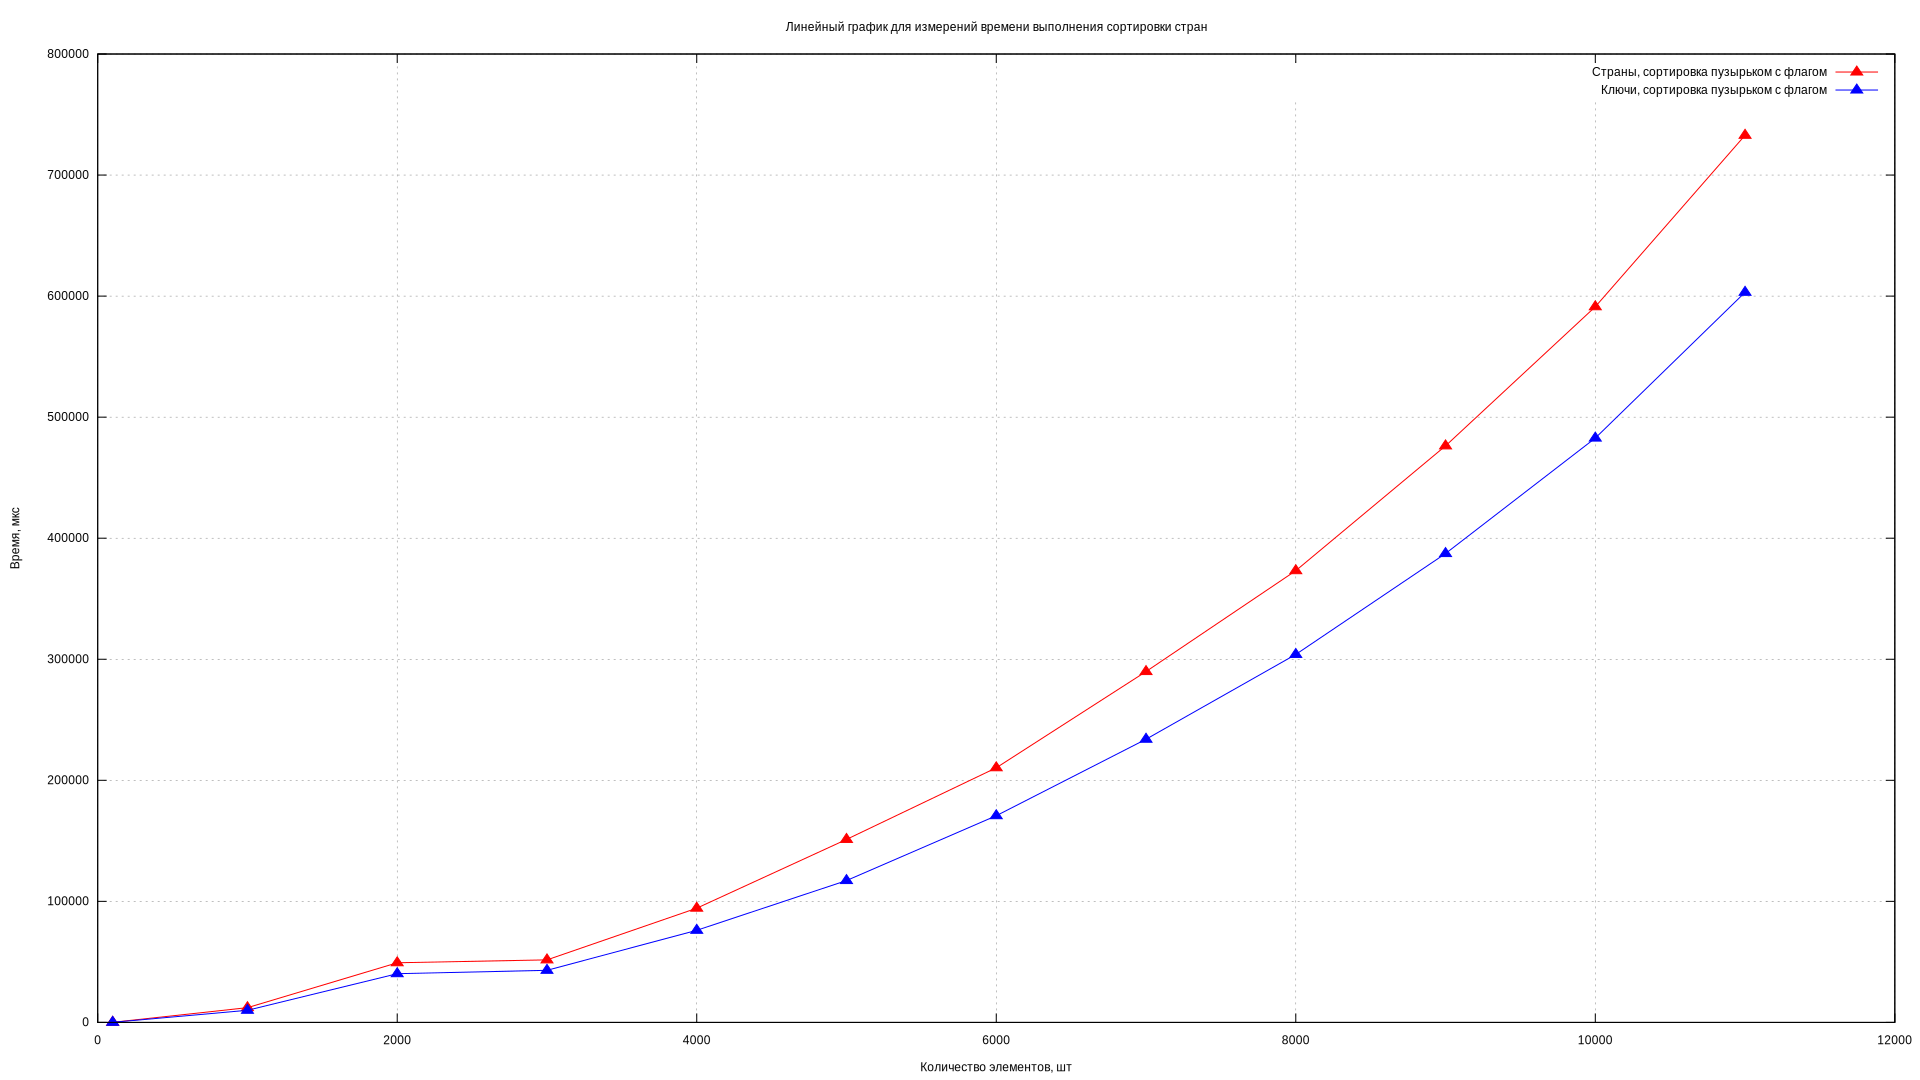
\includegraphics[width=0.94\textwidth]{img/linear_time_flag_buble.jpg}
	\captionsetup{font=footnotesize}
	\caption{Зависимость времени между сортировкой стран и ключей при сортировке пузырьком с флагом}
	\label{fig:02}
\end{figure}

\begin{table}[H]
	\begin{longtable}{|c|c|c|}
		\hline
		\makecell{Кол-во элементов} & \makecell{Время, мкс} & \makecell{Память, байт} \\
		\hline
		\makecell{1000}  & \makecell{23 028}   & \makecell{80 000}  \\
		\hline
		\makecell{4000}  & \makecell{94 265}   & \makecell{320 000} \\
		\hline
		\makecell{8000}  & \makecell{378 553}  & \makecell{640 000} \\
		\hline
		\makecell{11 000} & \makecell{717 998} & \makecell{880 000} \\
		\hline
	\end{longtable}
	\caption{Сортировка  таблицы пузырьком с флагом}
\end{table}


\begin{table}[H]
	\begin{longtable}{|c|c|c|}
		\hline
		\makecell{Кол-во элементов} & \makecell{Время, мкс} & \makecell{Память, байт} \\
		\hline
		\makecell{1000}  & \makecell{10018}     & \makecell{24 000}  \\
		\hline
		\makecell{4000}  & \makecell{77 359}   & \makecell{96 000}  \\
		\hline
		\makecell{8000}  & \makecell{310 965}  & \makecell{192 000} \\
		\hline
		\makecell{11 000} & \makecell{590 672}  & \makecell{264 000} \\
		\hline
	\end{longtable}
	\caption{Сортировка ключей пузырьком с флагом}
\end{table}

\textbf{Дополнительные графики}
\begin{figure}[H]
	\centering
	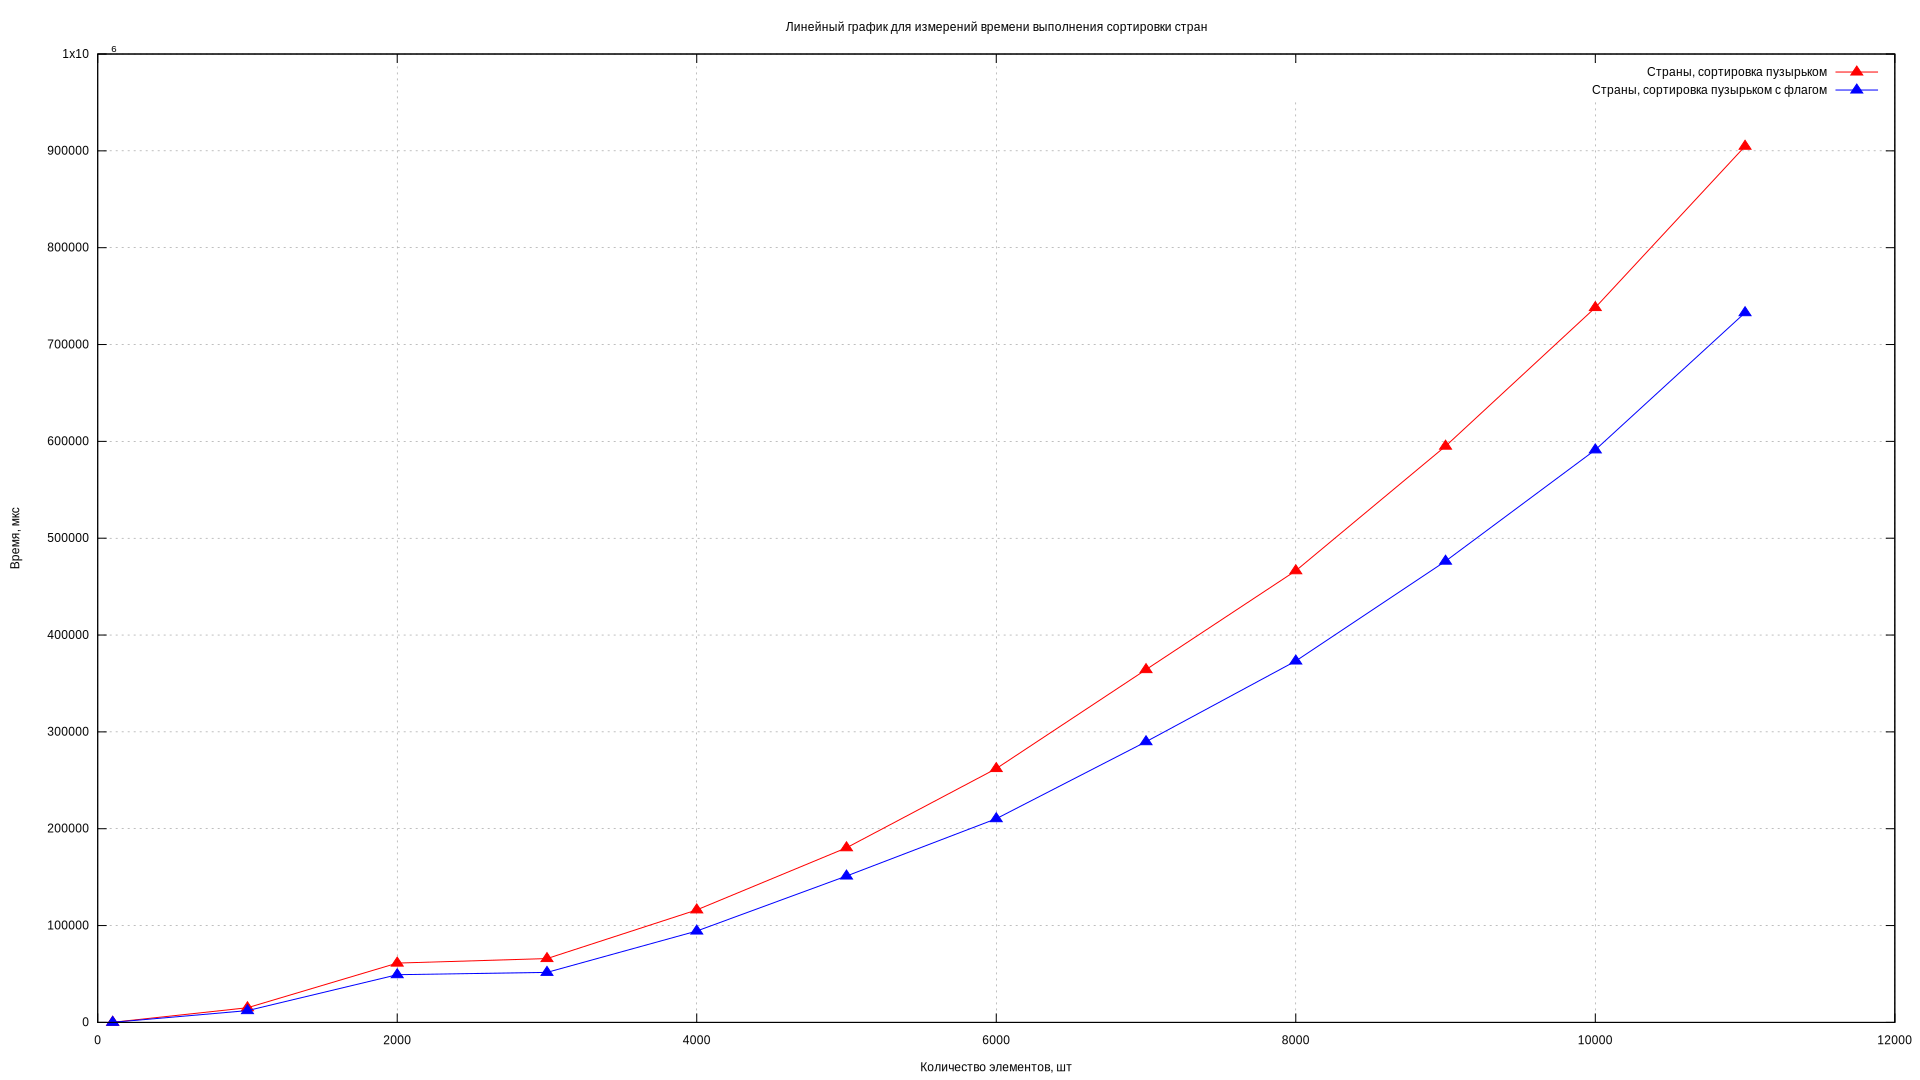
\includegraphics[width=1\textwidth]{img/linear_time_together_countries.jpg}
	\captionsetup{font=footnotesize}
	\caption{Зависимость времени между разным способом сортировки стран}
	\label{fig:03}
\end{figure}

\begin{figure}[H]
	\centering
	\includegraphics[width=1\textwidth]{img/linear_time_together_keys.jpg}
	\captionsetup{font=footnotesize}
	\caption{Зависимость времени между разным способом сортировки ключей}
	\label{fig:04}
\end{figure}


\subsection{Выводы исследования}
Как видно из полученных данных, использование ключей сокращает потребление памяти примерно на 70\%, а улучшение производительности по времени при сортировке ключей составляет около 20\%.
